% ==========================================
% BAB IV PERANCANGAN
% ==========================================
\chapter{PERANCANGAN}
\label{chap:perancangan}

Bab ini menjelaskan rancangan sistem \textit{Retrieval-Augmented Generation Large Language Model} (RAG-LLM) untuk mengurangi halusinasi pada tanya jawab biomedis. Rancangan ini menggabungkan tiga \textit{pipeline} utama, yaitu \textit{indexing}, \textit{retrieval}, dan \textit{generation}, yang dilengkapi dengan dua teknik mitigasi pilihan, yaitu \textit{query rewriting} (QR) dan \textit{context reranking} (CR). Bab ini juga menjelaskan pilihan model yang dipakai, daftar konfigurasi yang dibandingkan, serta nilai \textit{hyperparameter} dalam eksperimen.

% ==========================================
\section{Gambaran Umum Solusi}
\label{sec:gambaran-umum-solusi}

Sistem yang dirancang menggunakan pendekatan \textbf{hybrid retrieval}. Pendekatan ini menggabungkan dua jenis pencarian dokumen, yaitu pencarian berbasis kata kunci (BM25) dan pencarian berbasis kemiripan makna (\textit{dense embeddings}), lalu menggabungkan hasilnya melalui metode \textit{Reciprocal Rank Fusion} (RRF). Kedua jenis pencarian ini saling melengkapi: BM25 unggul saat mencari istilah biomedis tertentu seperti nama obat, gen, atau penyakit, sedangkan \textit{dense retrieval} mampu menemukan dokumen yang maknanya mirip walaupun kata yang dipakai berbeda.

Di atas dasar \textit{hybrid retrieval} tersebut, sistem menambahkan dua teknik mitigasi halusinasi sebagai pilihan:

\begin{enumerate}[1.]
  \item \textbf{\textit{Query Rewriting} (QR)}, yaitu modul \textit{Large Language Model} (LLM) yang menulis ulang pertanyaan pengguna sebelum dikirim ke \textit{pipeline retrieval}. Tujuannya adalah memperluas istilah medis dan membakukan singkatan agar pencarian lebih tepat. Modul ini bekerja \textit{sebelum} \textit{retrieval}.
  \item \textbf{\textit{Context Reranking} (CR)}, yaitu model \textit{cross-encoder} yang mengurutkan ulang 20 dokumen kandidat hasil RRF dan memilih lima dokumen yang paling relevan untuk diteruskan ke tahap \textit{generation}. Modul ini bekerja \textit{setelah} \textit{retrieval}.
\end{enumerate}

Gambaran umum sistem dapat dilihat pada Gambar~\ref{fig:bab4-master}.

\begin{figure}[H]
  \centering
  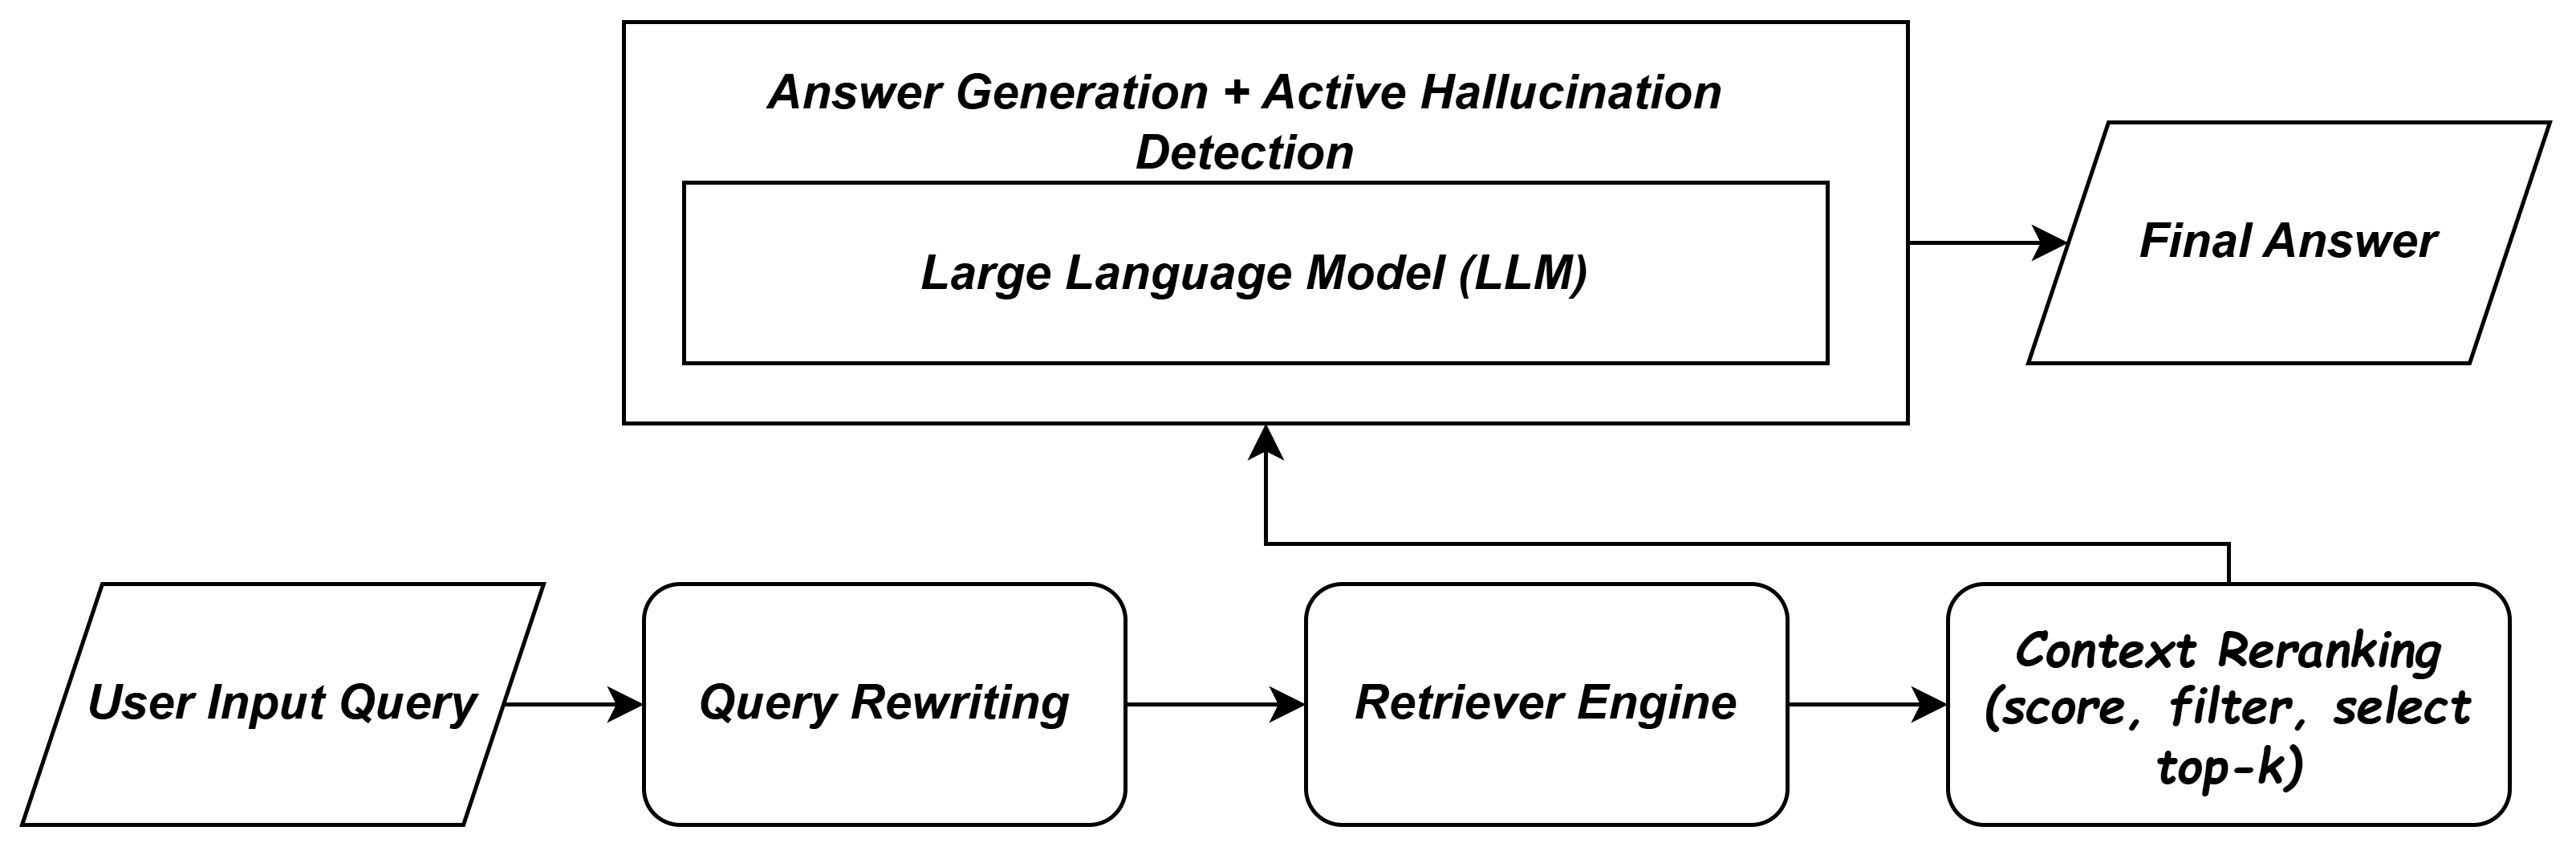
\includegraphics[width=0.95\textwidth]{image/flowsolusi.png}
  \caption[Diagram alur sistem RAG-LLM untuk mitigasi halusinasi]{Diagram alur sistem RAG-LLM untuk mitigasi halusinasi}
  \label{fig:bab4-master}
\end{figure}

% ==========================================
\section{Tahapan Perancangan Sistem}
\label{sec:tahapan-perancangan}

Tahap perancangan sistem dibagi menjadi empat bagian, yaitu \textit{data preparation}, \textit{indexing pipeline}, \textit{retrieval pipeline}, dan \textit{generation pipeline}. Masing-masing dijelaskan pada subbab berikut.

% ==========================================
\subsection{\textit{Data Preparation}}
\label{subsec:data-preparation}

Sumber data yang digunakan adalah \textbf{PubMedQA} bagian \texttt{pqa\_labeled}, yaitu kumpulan data berisi 1.000 pasangan tanya jawab biomedis yang sudah diberi label oleh ahli. Dari 1.000 pasangan tersebut, 500 sampel pertama dipilih untuk evaluasi dengan urutan tetap (\textit{seed} 42) agar hasil dapat diulang. Setiap entri PubMedQA sudah memuat artikel yang dipecah menjadi beberapa segmen sesuai struktur asli artikel ilmiah, yaitu \texttt{BACKGROUND}, \texttt{METHODS}, \texttt{RESULTS}, dan \texttt{CONCLUSIONS}. Cara pemecahan artikel ini disebut \textit{document-based chunking} dan dipertahankan apa adanya, karena pemecahan per bagian sudah menjaga makna setiap segmen tetap utuh dan ukurannya cukup seimbang (rata-rata 200 sampai 400 token per segmen).

Setelah seluruh sampel diproses, korpus akhir berisi \textbf{1.706 segmen dokumen} yang berasal dari 500 artikel sumber. Setiap segmen disimpan beserta metadata berikut: \texttt{pubid} (identitas artikel), \texttt{section\_label} (label bagian artikel), \texttt{question} (pertanyaan terkait artikel), \texttt{answer} (jawaban panjang), serta \texttt{decision} (label yes, no, atau maybe). Contoh hasil \textit{chunking} ditunjukkan pada Tabel~\ref{tbl:chunking-pubmedqa}.

\begin{table}[H]
\centering
\caption[Contoh hasil document-based chunking pada korpus PubMedQA]{Contoh hasil \textit{document-based chunking} pada korpus PubMedQA}
\label{tbl:chunking-pubmedqa}
\begin{tabularx}{\textwidth}{|c|c|X|c|}
\hline
\textbf{pubid} & \textbf{section} & \textbf{content (potongan teks)} & \textbf{decision} \\ \hline
21645374 & BACKGROUND & Programmed cell death is the regulated death of cells within an organism\ldots & yes \\ \hline
21645374 & METHODS & Cells of various stages were dissected from window stage leaves\ldots & yes \\ \hline
21645374 & RESULTS & Mitochondria were highly dynamic during early stages of PCD\ldots & yes \\ \hline
\end{tabularx}
\end{table}

Selain pemecahan dokumen, dilakukan pula proses \textit{tokenization} khusus untuk indeks BM25. \textit{Tokenizer} yang dipakai melakukan tiga langkah, yaitu (1) mengubah seluruh karakter menjadi huruf kecil, (2) menghapus tanda baca dengan ekspresi reguler \texttt{[\textasciicircum a-zA-Z0-9$\backslash$s]}, dan (3) memisahkan token berdasarkan spasi. \textit{Tokenization} ini berbeda dari \textit{embedding} semantik karena BM25 memerlukan token terpisah untuk menghitung \textit{term frequency}.

% ==========================================
\subsection{\textit{Indexing Pipeline}}
\label{subsec:indexing-pipeline}

\textit{Indexing pipeline} bertugas mengubah seluruh segmen dokumen menjadi dua bentuk indeks paralel yang akan dipakai oleh \textit{retrieval pipeline}. Kedua indeks dibangun satu kali saja dan disimpan secara persisten agar eksperimen berikutnya tidak perlu mengulang proses \textit{embedding}. Detail aliran proses ditunjukkan pada Gambar~\ref{fig:bab4-indexing}.

\begin{figure}[H]
  \centering
  \fbox{\parbox{0.9\textwidth}{\centering\vspace{1cm}\textit{[Placeholder: bab4\_indexing\_pipeline.png. Detail Indexing Pipeline dengan dua jalur, yaitu jalur sparse (BM25 Tokenization, BM25Okapi, dan pubmedqa\_bm25.pkl) serta jalur dense (Embedding Model, Vector Embeddings, dan ChromaDB)]}\vspace{1cm}}}
  \caption[Detail aliran proses Indexing Pipeline]{Detail aliran proses \textit{Indexing Pipeline}}
  \label{fig:bab4-indexing}
\end{figure}

\textbf{Jalur sparse (BM25)}. Setiap segmen di-\textit{tokenize} dengan \textit{tokenizer} BM25 (lihat Subbab~\ref{subsec:data-preparation}). Seluruh daftar token kemudian dibangun menjadi indeks BM25Okapi melalui pustaka \texttt{rank\_bm25}. Hasilnya disimpan ke berkas \texttt{pubmedqa\_bm25.pkl} yang berisi objek BM25Okapi dan daftar dokumen dalam urutan asli.

\textbf{Jalur dense (\textit{embeddings})}. Setiap segmen diubah menjadi vektor menggunakan model \textit{embedding} sesuai konfigurasi (lihat Subbab~\ref{subsec:opsi-model}). Vektor tersebut kemudian disimpan dalam basis data vektor \textbf{ChromaDB} dengan mode \textit{persistent client}. Konfigurasi basis data vektor ditunjukkan pada Tabel~\ref{tbl:vector-db-spec}.

\begin{table}[H]
\centering
\caption[Spesifikasi basis data vektor untuk Dense Retrieval]{Spesifikasi basis data vektor untuk \textit{Dense Retrieval}}
\label{tbl:vector-db-spec}
\begin{tabular}{|p{3.2cm}|p{4.2cm}|c|p{3.0cm}|}
\hline
\textbf{Embedder} & \textbf{Path persisten} & \textbf{Dim.} & \textbf{Distance metric} \\ \hline
nomic-embed-text & \texttt{pubmedqa\_\allowbreak chroma\_llama/} & 768 & cosine (HNSW) \\ \hline
text-embedding-3-small & \texttt{pubmedqa\_chroma/} & 1536 & cosine (HNSW) \\ \hline
\end{tabular}
\end{table}

\textit{Cosine similarity} dipilih sebagai \textit{distance metric} karena merupakan metrik standar untuk model \textit{embedding} teks. Algoritma indeks \textit{Hierarchical Navigable Small World} (HNSW) dipakai agar pencarian \textit{nearest neighbor} berjalan cepat walaupun jumlah vektor besar.

% ==========================================
\subsection{\textit{Retrieval Pipeline}}
\label{subsec:retrieval-pipeline}

\textit{Retrieval pipeline} bertugas mengambil dokumen yang paling relevan dengan pertanyaan pengguna. Sistem ini dirancang dalam empat varian sesuai kombinasi penggunaan QR dan CR. Empat varian tersebut dibahas berurutan pada subbab di bawah ini.

\subsubsection{Konfigurasi \textit{Baseline} (Hybrid Retrieval)}

Konfigurasi dasar memakai \textbf{hybrid retrieval} murni tanpa QR maupun CR. Aliran proses ditunjukkan pada Gambar~\ref{fig:bab4-baseline}.

\begin{figure}[H]
  \centering
  \fbox{\parbox{0.9\textwidth}{\centering\vspace{1cm}\textit{[Placeholder: bab4\_retrieval\_baseline.png. Pertanyaan pengguna diproses paralel oleh BM25 Search top-50 dan Dense Search top-50, lalu digabungkan dengan RRF Fusion (k=60), dan menghasilkan Top-5 Chunks]}\vspace{1cm}}}
  \caption[Detail aliran proses Retrieval Pipeline konfigurasi Baseline]{Detail aliran proses \textit{Retrieval Pipeline} konfigurasi \textit{Baseline}}
  \label{fig:bab4-baseline}
\end{figure}

Proses \textit{retrieval} pada konfigurasi ini terdiri dari tiga langkah:

\begin{enumerate}[1.]
  \item \textbf{BM25 Search top-50}. Pertanyaan di-\textit{tokenize} dengan \textit{tokenizer} BM25 yang sama seperti pada \textit{indexing}. Setelah itu sistem menghitung skor BM25 terhadap seluruh segmen pada indeks \textit{sparse} dan mengambil 50 segmen dengan skor tertinggi.
  \item \textbf{Dense Search top-50}. Pertanyaan diubah menjadi vektor oleh model \textit{embedding} yang sama dengan \textit{indexing}. ChromaDB kemudian mengembalikan 50 segmen dengan \textit{cosine similarity} tertinggi.
  \item \textbf{RRF Fusion}. Kedua daftar peringkat (BM25 dan Dense) digabungkan menggunakan rumus \textit{Reciprocal Rank Fusion} (RRF):
  \[
    \mathrm{RRF}(d) = \sum_{r \in R} \frac{1}{k + \mathrm{rank}_r(d)}
  \]
  dengan $k = 60$ (nilai standar literatur~\parencite{cormack2009reciprocal}) dan $R$ adalah himpunan dua daftar peringkat. Lima segmen dengan skor RRF tertinggi diambil sebagai konteks akhir untuk \textit{generation pipeline}.
\end{enumerate}

\subsubsection{Konfigurasi + \textit{Query Rewriting} (QR)}

Konfigurasi QR menambahkan modul \textit{Query Rewriter} berbasis LLM \textit{sebelum} tahap \textit{hybrid retrieval}. Aliran proses ditunjukkan pada Gambar~\ref{fig:bab4-qr}.

\begin{figure}[H]
  \centering
  \fbox{\parbox{0.9\textwidth}{\centering\vspace{1cm}\textit{[Placeholder: bab4\_retrieval\_qr.png. Pertanyaan asli diproses oleh Query Rewriter (LLM, temp=0.3), menghasilkan Rewritten Query, lalu masuk ke BM25 Search dan Dense Search top-50, RRF Fusion, dan menghasilkan Top-5 Chunks. Catatan: tahap Generation tetap memakai pertanyaan asli.]}\vspace{1cm}}}
  \caption[Detail aliran proses Retrieval Pipeline + Query Rewriting]{Detail aliran proses \textit{Retrieval Pipeline} + \textit{Query Rewriting}}
  \label{fig:bab4-qr}
\end{figure}

\textit{Query Rewriter} menerima pertanyaan mentah dan menghasilkan versi yang sudah diperluas dengan istilah medis baku. Sebagai contoh, singkatan ``MI'' diperluas menjadi ``\textit{myocardial infarction}''. LLM yang sama dengan tahap \textit{generation} dipakai agar konsisten, namun dengan \textit{temperature} 0.3 untuk memberi sedikit ruang variasi parafrasa. \textbf{Pertanyaan hasil rewrite hanya dipakai untuk \textit{retrieval}}. Tahap \textit{generation} tetap memakai pertanyaan asli sehingga jawaban akhir menjawab pertanyaan pengguna apa adanya.

\subsubsection{Konfigurasi + \textit{Context Reranking} (CR)}

Konfigurasi CR mempertahankan \textit{hybrid retrieval} dasar, namun memperbanyak kandidat hasil RRF dari 5 menjadi \textbf{20 kandidat}, lalu mengurutkan ulang kandidat tersebut menggunakan model \textit{CrossEncoder}. Aliran proses ditunjukkan pada Gambar~\ref{fig:bab4-cr}.

\begin{figure}[H]
  \centering
  \fbox{\parbox{0.9\textwidth}{\centering\vspace{1cm}\textit{[Placeholder: bab4\_retrieval\_cr.png. Pertanyaan pengguna diproses paralel oleh BM25 Search dan Dense Search top-50, lalu RRF Fusion (k=60) mengambil 20 kandidat, kemudian CrossEncoder Reranker (ms-marco-MiniLM-L-6-v2) memilih Top-5 Chunks akhir]}\vspace{1cm}}}
  \caption[Detail aliran proses Retrieval Pipeline + Context Reranking]{Detail aliran proses \textit{Retrieval Pipeline} + \textit{Context Reranking}}
  \label{fig:bab4-cr}
\end{figure}

Model \textit{CrossEncoder} \texttt{ms-marco-\allowbreak MiniLM-L-6-v2} menerima pasangan pertanyaan dan dokumen, lalu mengeluarkan skor relevansi yang lebih akurat dibandingkan \textit{cosine similarity} pada \textit{dense retrieval}. Hal ini terjadi karena model membaca pertanyaan dan dokumen secara bersamaan dalam satu \textit{forward pass}. Lima segmen dengan skor tertinggi diambil sebagai konteks akhir.

\subsubsection{Konfigurasi + QR + CR}

Konfigurasi terakhir menggabungkan kedua teknik mitigasi, yaitu modul QR di awal \textit{pipeline} dan modul CR di akhir \textit{pipeline}. Aliran proses ditunjukkan pada Gambar~\ref{fig:bab4-qrcr}.

\begin{figure}[H]
  \centering
  \fbox{\parbox{0.9\textwidth}{\centering\vspace{1cm}\textit{[Placeholder: bab4\_retrieval\_qrcr.png. Pertanyaan pengguna diproses Query Rewriter, menghasilkan Rewritten Query, lalu BM25 dan Dense, RRF top-20, CrossEncoder Reranker, dan menghasilkan Top-5 Chunks. Tahap Generation tetap memakai pertanyaan asli.]}\vspace{1cm}}}
  \caption[Detail aliran proses Retrieval Pipeline + QR + CR]{Detail aliran proses \textit{Retrieval Pipeline} + QR + CR}
  \label{fig:bab4-qrcr}
\end{figure}

Konfigurasi ini diharapkan memberikan kualitas \textit{retrieval} terbaik karena memperbaiki dua titik penting sekaligus, yaitu kualitas pertanyaan di awal melalui QR dan kualitas pemilihan konteks di akhir melalui CR.

% ==========================================
\subsection{\textit{Generation Pipeline}}
\label{subsec:generation-pipeline}

\textit{Generation pipeline} menyusun \textit{prompt} berdasarkan pertanyaan asli pengguna dan lima segmen konteks hasil \textit{retrieval}. \textit{Prompt} tersebut kemudian dikirim ke LLM untuk menghasilkan jawaban. \textit{Pipeline} ini sama untuk seluruh empat konfigurasi \textit{retrieval}.

\textit{Prompt template} dirancang dengan tiga prinsip utama, yaitu (1) instruksi tegas agar LLM hanya memakai informasi dari konteks yang diberikan, (2) panduan agar LLM memilih label \texttt{yes}, \texttt{no}, atau \texttt{maybe} secara konsisten, dan (3) format keluaran yang teratur agar label mudah diekstrak. Detail \textit{prompt template} ditunjukkan pada Tabel~\ref{tbl:prompt-generation}.

\begin{table}[H]
\centering
\caption[Prompt template untuk Generation Pipeline]{\textit{Prompt template} untuk \textit{Generation Pipeline}}
\label{tbl:prompt-generation}
\begin{tabular}{|p{12.5cm}|}
\hline
\textbf{GENERATION\_PROMPT} \\ \hline
\ttfamily\footnotesize
You are a medical research assistant. Answer a biomedical yes/no/maybe question based solely on the provided scientific abstracts.\par\medskip
Context from medical literature:\par
\{context\}\par\medskip
Question: \{question\}\par\medskip
Instructions:\par
\quad\quad - Carefully read the context and assess whether it supports or refutes the question.\par
\quad\quad - Provide a brief explanation (2 to 3 sentences) using ONLY the information above.\par
\quad\quad - End your response with EXACTLY ONE of these words on its own line: yes, no, or maybe.\par
\quad\quad\quad\quad - yes\quad\,: the evidence supports the hypothesis, even if not perfectly conclusive\par
\quad\quad\quad\quad - no\quad\,\,: the evidence refutes or does not support the hypothesis\par
\quad\quad\quad\quad - maybe : ONLY if the evidence is directly contradictory, or contains no relevant info\par
\quad\quad - IMPORTANT: If evidence leans in one direction, choose yes or no.\par\medskip
Answer: \\ \hline
\end{tabular}
\end{table}

Setelah jawaban dihasilkan, fungsi \textit{label extractor} membaca baris terakhir keluaran LLM dan mencocokkannya dengan tiga label valid (\texttt{yes}, \texttt{no}, atau \texttt{maybe}). Apabila format keluaran tidak sesuai, label \texttt{maybe} dipakai sebagai cadangan agar tidak ada sampel yang hilang.

% ==========================================
\section{Konfigurasi Model}
\label{sec:konfigurasi-model}

Sistem RAG-LLM membutuhkan tiga jenis model, yaitu \textit{embedding model} untuk \textit{dense retrieval}, \textit{reranker model} untuk \textit{context reranking}, dan \textit{Large Language Model} (LLM) untuk \textit{query rewriting} dan pembuatan jawaban. Subbab ini menjelaskan opsi model yang dipertimbangkan dan daftar konfigurasi yang akan dibandingkan.

% ==========================================
\subsection{Opsi Model}
\label{subsec:opsi-model}

Pemilihan model didasarkan pada empat kriteria, yaitu (1) kualitas keluaran pada bidang biomedis, (2) ketersediaan API atau model lokal yang stabil, (3) biaya operasional yang sesuai dengan anggaran tugas akhir, dan (4) kemampuan menangani konteks yang panjang. Berdasarkan kriteria tersebut, dipilih opsi model yang ditunjukkan pada Tabel~\ref{tbl:opsi-model}.

\begin{table}[H]
\centering
\caption{Opsi model dalam implementasi sistem RAG-LLM}
\label{tbl:opsi-model}
\begin{tabularx}{\textwidth}{|c|p{2.5cm}|>{\raggedright\arraybackslash}X|p{3.5cm}|}
\hline
\textbf{No.} & \textbf{Jenis Model} & \textbf{Opsi Model} & \textbf{Penyedia} \\ \hline
1 & \textit{Embedding} & nomic-embed-text (768d) & Ollama (lokal) \\ \cline{3-4}
  &                    & text-embedding-3-small (1536d) & OpenAI API \\ \hline
2 & \textit{Reranker}  & ms-marco-MiniLM-L-6-v2 & SentenceTransformers \\ \hline
3 & LLM Generator      & llama-3.3-70b-instruct & OpenRouter API \\ \cline{3-4}
  &                    & gpt-4.1-mini & OpenAI API \\ \hline
\end{tabularx}
\end{table}

\textbf{Justifikasi pemilihan.} Model \textit{embedding} \texttt{nomic-embed-text} dipilih sebagai pasangan model Llama karena keduanya dapat dijalankan secara lokal melalui Ollama, sehingga tidak ada biaya API maupun keterlambatan jaringan. Model \textit{embedding} \texttt{text-embedding-3-small} dipilih untuk pasangan GPT-4.1-mini karena keduanya berasal dari penyedia yang sama, yaitu OpenAI, dan terbukti cocok dipakai bersama dalam berbagai studi RAG. Model \textit{reranker} \texttt{ms-marco-MiniLM-L-6-v2} dipilih karena ukurannya kecil (22 MB), berjalan cepat di CPU, dan secara umum kuat untuk \textit{passage reranking} lintas bidang. Untuk LLM generator, Llama 3.3 70B dipilih sebagai contoh model \textit{open-source} berukuran besar yang diakses melalui API OpenRouter, sedangkan GPT-4.1-mini dipilih sebagai contoh model \textit{closed-source} yang murah dengan kualitas mengikuti instruksi yang baik.

% ==========================================
\subsection{Matriks Konfigurasi yang Dibandingkan}
\label{subsec:matriks-konfigurasi}

Untuk mengukur kontribusi setiap teknik mitigasi terhadap penurunan halusinasi pada masing-masing LLM, dilakukan perbandingan \textbf{delapan konfigurasi} sebagai hasil kombinasi empat teknik \textit{retrieval} (\textit{Baseline}, +QR, +CR, dan +QR+CR) dengan dua LLM utama (Llama 3.3 70B dan GPT-4.1-mini). Daftar konfigurasi ditunjukkan pada Tabel~\ref{tbl:matriks-konfigurasi}.

\begin{table}[H]
\centering
\caption{Matriks konfigurasi sistem RAG-LLM yang dibandingkan}
\label{tbl:matriks-konfigurasi}
\begin{tabular}{|p{3cm}|p{2.6cm}|p{3cm}|c|c|}
\hline
\textbf{Konfigurasi} & \textbf{LLM Generator} & \textbf{Embedder} & \textbf{QR} & \textbf{CR} \\ \hline
baseline\_llama  & Llama 3.3 70B & nomic-embed-text & Tidak & Tidak \\ \hline
qr\_llama        & Llama 3.3 70B & nomic-embed-text & Ya    & Tidak \\ \hline
cr\_llama        & Llama 3.3 70B & nomic-embed-text & Tidak & Ya    \\ \hline
qr\_cr\_llama    & Llama 3.3 70B & nomic-embed-text & Ya    & Ya    \\ \hline
baseline\_openai & GPT-4.1-mini  & text-embedding-3-small & Tidak & Tidak \\ \hline
qr\_openai       & GPT-4.1-mini  & text-embedding-3-small & Ya    & Tidak \\ \hline
cr\_openai       & GPT-4.1-mini  & text-embedding-3-small & Tidak & Ya    \\ \hline
qr\_cr\_openai   & GPT-4.1-mini  & text-embedding-3-small & Ya    & Ya    \\ \hline
\end{tabular}
\end{table}

Seluruh konfigurasi memakai \textit{retriever} dasar yang sama (\textbf{hybrid BM25 dan Dense melalui RRF}), sehingga perbedaan hasil dapat langsung dikaitkan dengan kontribusi teknik QR, CR, atau kombinasi keduanya. Hasil eksperimen untuk seluruh konfigurasi dibahas pada Bab~\ref{chap:evaluasi}.

% ==========================================
\section{Hyperparameter dan Setup Eksperimen}
\label{sec:hyperparameter-setup}

Subbab ini menjelaskan nilai \textit{hyperparameter} yang dipakai pada setiap komponen \textit{pipeline} serta setup evaluasi. Seluruh nilai dipilih berdasarkan rekomendasi literatur atau hasil studi pustaka pada Bab~\ref{chap:studi}, dan ditetapkan sama untuk seluruh delapan konfigurasi agar perbandingan bersifat setara. Daftar lengkap ditunjukkan pada Tabel~\ref{tbl:hyperparameter}.

\begin{table}[H]
\centering
\caption{Hyperparameter dan setup eksperimen}
\label{tbl:hyperparameter}
\begin{tabular}{|p{3cm}|p{4.2cm}|c|p{3.5cm}|}
\hline
\textbf{Komponen} & \textbf{Parameter} & \textbf{Nilai} & \textbf{Catatan} \\ \hline
BM25     & top-K            & 50    & Sebelum RRF fusion \\ \hline
Dense    & top-K            & 50    & Sebelum RRF fusion \\ \hline
RRF      & konstanta $k$    & 60    & Standar literatur \\ \hline
Final    & top-K (tanpa CR) & 5     & Diteruskan ke generator \\ \hline
CR       & jumlah kandidat  & 20    & Sebelum reranking \\ \hline
CR       & top-K final      & 5     & Setelah reranking \\ \hline
Generator & temperature     & 0.0   & Keluaran konsisten \\ \hline
Generator & max\_tokens     & 300   & Cukup untuk 2 sampai 3 kalimat dan label \\ \hline
QR       & temperature      & 0.3   & Variasi parafrasa terbatas \\ \hline
QR       & max\_tokens      & 150   & Cukup untuk \textit{rewritten query} \\ \hline
Sampling & jumlah sampel    & 500   & Konsisten antar konfigurasi \\ \hline
Sampling & seed             & 42    & Untuk reproduktibilitas \\ \hline
\end{tabular}
\end{table}

\textbf{Evaluator.} Setiap konfigurasi dievaluasi dengan metrik kuantitatif dalam dua tahap. Tahap pertama (\textit{Phase 1}) menghitung \textbf{Label Accuracy} dengan membandingkan label prediksi sistem (\texttt{yes}, \texttt{no}, atau \texttt{maybe}) terhadap \textit{ground truth} PubMedQA. Tahap kedua (\textit{Phase 2}) memakai \textbf{evaluator kustom 4 metrik} yang merupakan adaptasi dari kerangka RAGAS dengan jaminan zero-NaN, yaitu (1) \textit{faithfulness} (kesesuaian klaim jawaban dengan konteks), (2) \textit{context recall} (cakupan informasi referensi oleh konteks), (3) \textit{answer relevancy} (relevansi jawaban terhadap pertanyaan), dan (4) \textit{context precision} (ketepatan konteks dalam mendukung jawaban). Detail metrik dan implementasinya dijelaskan pada Bab~\ref{chap:evaluasi}.

% ==========================================
\section{Pengembangan Lanjutan}
\label{sec:future-work}

Beberapa arah pengembangan dipertimbangkan namun berada di luar cakupan eksperimen utama tugas akhir ini. Pengembangan tersebut dijelaskan sebagai \textit{future work} berikut:

\begin{enumerate}[1.]
  \item \textbf{\textit{Active Hallucination Detection} (AHD)}, yaitu penambahan modul setelah tahap \textit{generation} yang menilai tingkat keyakinan keluaran LLM. Apabila ada bagian yang berpotensi halusinatif, modul ini akan memperbaikinya secara terbatas pada bagian yang bermasalah (\textit{span-level repair}) atau menghasilkan ulang seluruh jawaban dengan instruksi yang lebih ketat (\textit{strict regeneration}). Pendekatan ini menjanjikan untuk menutup kelemahan tahap \textit{generation} yang tidak dapat diatasi oleh QR maupun CR.
  \item \textbf{Validasi lintas penyedia (\textit{multi-provider})}, yaitu uji coba memakai model Claude Haiku 4.5 dari Anthropic pada konfigurasi \textit{baseline}. Uji coba ini bertujuan memvalidasi sifat \textit{provider-agnostic} dari \textit{pipeline}. Pembahasan hasil uji coba tersebut disertakan pada Bab~\ref{chap:evaluasi} sebagai studi tambahan.
  \item \textbf{Validasi lintas bidang (\textit{cross-domain})}, yaitu evaluasi pada dataset di luar bidang biomedis seperti ASQA atau Natural Questions. Tujuannya adalah menguji apakah keunggulan teknik QR dan CR konsisten saat dipakai pada bidang lain.
\end{enumerate}

Ketiga pengembangan tersebut dapat menjadi titik awal penelitian lanjutan untuk memperluas kontribusi tugas akhir ini.
